%------------------------------------%
% Début Partie Azarias				%
%------------------------------------%
\part{System design}

\chapter{User interface design}
Because the project was created with Qt, and Qt adapt its interface depending on the OS it's running on, there is no 'global' user interface. However, the layout is always the same and so is the content. The following screenshots will show the user interface as it is on Linux, more precisely Ubuntu. Currently, QTypingTest is available on Ubuntu and windows.\\
When the user starts the software, he's directly directed on the homepage, figure \ref{homepage-logout} where he can either create a new profile or connect himself to his own existing profile. The buttons allowing to go through the differents part of the software are disabled as long as no one is connected. A list of the existing user is displayed and the user just has to click on his alias to be considered as connected(figure \ref{homepage-login}. He can then go through the differents part of the user interface. 
\begin{figure}[H]
  \centering
  \begin{minipage}[b]{0.45\textwidth}
    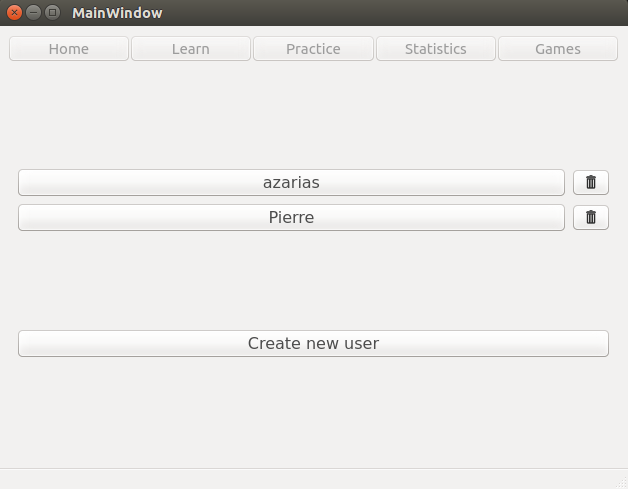
\includegraphics[width=\textwidth]{images/homepage_logout.png}
    \caption{Defaults homepage.}
    \label{homepage-logout}
  \end{minipage}
  \hfill
  \begin{minipage}[b]{0.45\textwidth}
    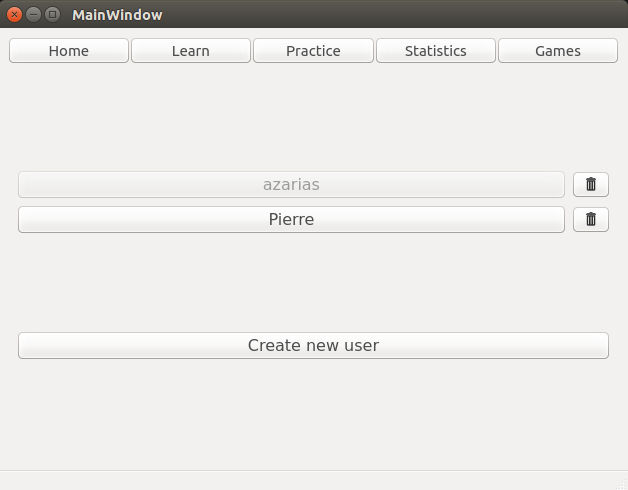
\includegraphics[width=\textwidth]{images/homepage_login.png}
    \caption{User connected.}
    \label{homepage-login}
  \end{minipage}
\end{figure}
A user can also delete his profile by clicking on the trash icon. \\
The purpose of the login system was not to be secured. Since this software is made for private use, and that it does not contain any sensible informations, the group decided to focus on the software itself and to do not spend to much time on the login system. \\
On the top of the window, there are five buttons.
\begin{itemize}
	\item Home. This button, when triggered, shows the homepage, but does not disconnect the user.
	\item Learn. This show the main part of the project. The page where the user has a list of the differents letters to learn in an certain order.
	\item Practice. On this page, the user can choose differents mode of practice.
	\item Statistics. Here, the user can see his statics.
	\item Games. Some simple games developed to learn the fun way to type.
\end{itemize}


\begin{figure}[H]
	\centering
	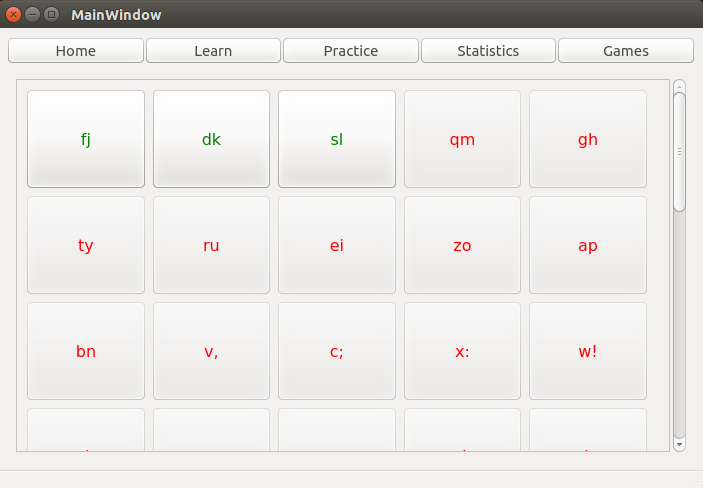
\includegraphics[width=0.7\textwidth]{images/page-learn.png}
	\caption{Learn page}
	\label{page-learn}
\end{figure}

The learn page (figure \ref{page-learn}) the user can see all the exercises to come. He must succeed to them one by one. And should realize a minimum score the be able to unlock the next exercise. When clicking on a button, a dialog is shown and the user can start a new exercise.

\begin{figure}[H]
	\centering
	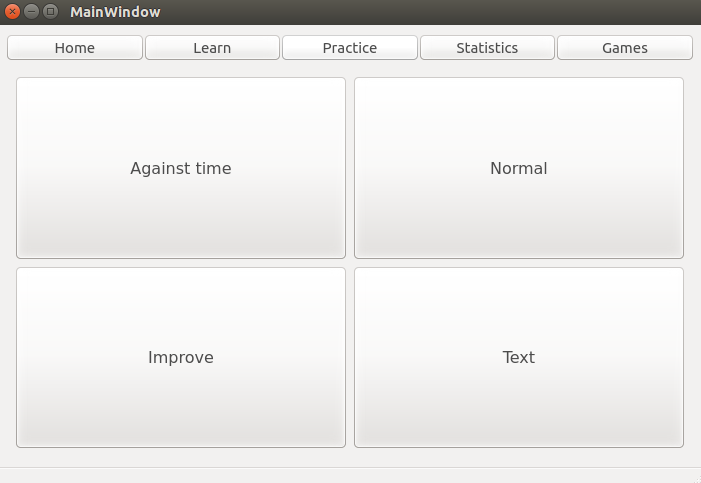
\includegraphics[width=0.7\textwidth]{images/page-practice.png}
	 \caption{Practice page}
	 \label{page-practice}
\end{figure}

The practice page  (figure \ref{page-practice}) has four buttons. On for each differents type of practice. The final 'form' of each practice is always the same : a dialog with text to type. What's changing is the content of the dialog.\\
The differents rules for each types of practice are 
\begin{enumerate}
	\item[Against time :] The user must type the most words in one minute. At the end of this time, his number of words per minute is shown.
	\item[Normal :] The user has two 'pages' of random words to type. Thanks to the powerful language system of Qt, the displayed words may change depending on the user's computer language. For the moment, only english and french is supporter.
	\item[Improve :] This practice will check what is the user's worst letters and create a special exercise containing these letters.
	\item[Text :] In this practice, the user will have to type an existing text. The chosen text are the 'classical' authors such as George Orwell. Once again thanks to Qt, the language of the text may vary depending on the user's computer language. The default language being english. 
\end{enumerate}

\textit{The statistics page was not made yet}

\begin{figure}[H]
	\centering
	\includegraphics[width=0.7\textwidth]{images/page-game.png}
	 \caption{Game page}
	 \label{page-game}
\end{figure}

The game page contains a single button. This button launches a dialog where the user see what letters is associated with what finger on the keyboard.

\begin{figure}[H]
  \centering
  \begin{minipage}[b]{0.45\textwidth}
    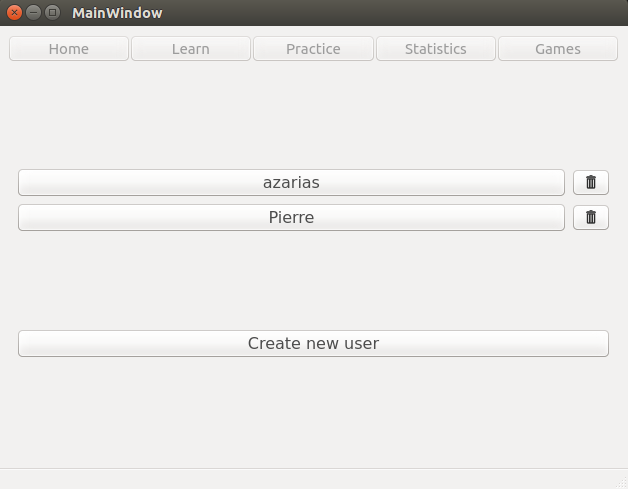
\includegraphics[width=\textwidth]{images/homepage_logout.png}
    \caption{Defaults homepage.}
    \label{homepage-logout}
  \end{minipage}
  \hfill
  \begin{minipage}[b]{0.45\textwidth}
    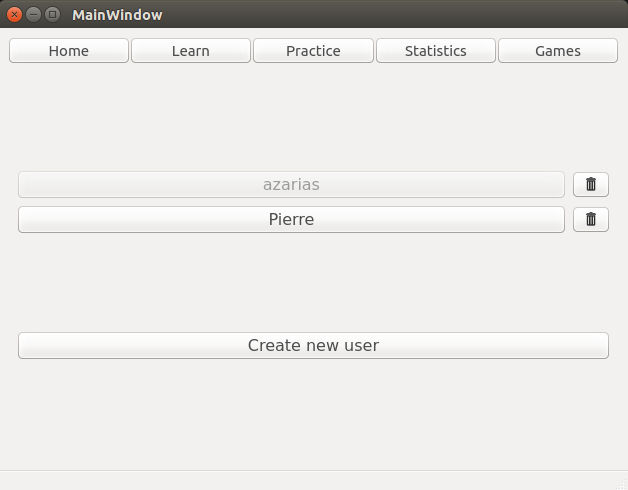
\includegraphics[width=\textwidth]{images/homepage_login.png}
    \caption{User connected.}
    \label{homepage-login}
  \end{minipage}
\end{figure}


\section{Qt features}
Qt features

\chapter{Functional Design}
Functional Design

\section{Structure of the system}
Structure of the system

\section{Code walkthrough}
Code walkthrough


\chapter{Data design}
Data design
\part{System implementation}

\chapter{Building the software}
\section{First prototype}
The first prototype that the group presented to the first demo was giving an idea of the project. It was really fast to build and was containing only one window. On which the user could write down a text. It was a sort of 'proof of concept'. The purpose of this prototype was to demonstrate the main feature of the software and it was also a starting point for the group.\\
The first prototype was containing only two C++ classes. One for the whole window, and one for each row. Even if the prototype was working well, the interface was not very user-friendly and an offset could easily appear when the user was making too many mistakes.
Meaning that even if the prototype was working, a lot of work would be necessary to improve the user interface. \\
This prototype was also a sort of training for the group, it was the first window ever made with Qt. Because the group members didn't know anything about Qt, it was absolutely normal to have such a poor interface.

\section{Second prototype}
The second an actual prototype is a lot more evolved than the first prototype. There are more features, it's working better and it's more user-friendly. Of course, there is some improvements that remains possible.\\
However, the software is ready for production and can be used by anyone who wants to.\\
The second prototype started with a big improvement of the first prototype. The two lines : one for the text, and one for the text-field where the user can type were merged into a single one. So, as the user would type the text, the current character would be displayed in a certain color, the future characters would also be displayed as 'passed'. Therefore, the offset problem was solved. Thanks to the support of HTML in the label with Qt, the task was quite easy.\\
Now that the group had a functional and user-friendly base, they could start to work on the other parts of the project and use this base for differents features.\\
Here are the list of features that were developed on this base, by order of development :
\begin{enumerate}
	\item random-letters typing. Were the user has to type a random set of letters
	\item random-words typing. Were the user has to type real words
	\item text typing. Were the user has to type an existing text (written by great authors such as George Orwell)
	\item improvement. This exercise is using the statistics of the user to know what mistake is the more frequent
\end{enumerate}
All these differents exercise has its own class. But they also all inherit from the same base class to have access to the same resources such as a timer, a play/pause button, and a score a the end.\\
Then the group worked on different aspects of the main program, such as an interactive keyboard, the user's statistics and a homepage where a use can create its account, connect/disconnect.


\chapter{Current state of the software}
The current state of the software is complete. The software is available on \url{github.com} and can be downloaded for Linux or Windows. Anyone with a computer can download the software and start to learn how to type !
Even if the system is working well, the GUI is improvable. However, since the group is not design experts, they did as they could to create a usable software that does not hurt the eyes. And because the software is made up in C++, it's a bit harder than the web to stylize the interface. Even though Qt provides a CSS-like feature to change the style of every elements in a window.


\part{Testing}

\chapter{Unit testing}
Really early in the development of the software, it became obvious that some key features required unit testing.\\
Luckily Qt provides a way to easily and quickly create unit testing. All the tests of the projects are on the 'test' folder.\\
The tests for this projects were created for two main purpose :
\begin{enumerate}
	\item ensure that the feature are working as expected
	\item avoid compiling all the project for a single feature test
\end{enumerate}
Some test requires the GUI some does not. The hard part of the test was not to create them, it was to make the software testable. For example, a lots of features held on randomness. And it is not possible (or silly) to test randomness. This means, the less randomness, the more testable. Or pseudo-random features were testable.

\chapter{GUI testing}
GUI testing

\part{Usability - Users tasks}
Usability - Users tasks

\chapter{What can the user do}
What can the user do


\chapter{Efficiency and response times}
Efficiency and response times

\chapter{Overall aesthetic}
Overall aesthetic

\part{Conclusion and further work}
Conclusion and further work

\chapter{Project result}
Project result

\chapter{Possible improvements}
Possible improvements

\chapter{Further work}
Further work
%------------------------------------%
% Fin Partie Azarias					%
%------------------------------------%